\section{Dataset Artificial}
\label{sec:datasetArtificial}

El banco de animaciones en el que fueron buscados los gestos necesarios fue Mixamo. \footnote{Página web de Mixamo: \url{https://www.mixamo.com}}

Mixamo es una página web creada por Adobe en la que se encuentran de manera gratuita modelos con un \gls{rig} humanoide y animaciones para estos rigs, además de una funcionalidad que permite crear el \gls{rig} de un personaje que se suba a la página.
En la página hay un buscador en el que puedes buscar tipos de animaciones, pero como no es viable descargarse todas las animaciones de todos los gestos buscados se usó una herramienta para automatizarlo.

\subsection{Herramienta para descargarse animaciones de Mixamo de forma automática}

Esta herramienta se encontró en GitHub hecha por el usuario \textit{juanjo4martinez}\footnote{Enlace al perfil del creador de la herramienta \url{https://github.com/juanjo4martinez}}. La herramienta (mixamo-downloader\footnote{Enlace al repositorio de la herramienta \url{https://github.com/juanjo4martinez/mixamo-downloader}}) permite buscar y descargar animaciones de Mixamo de manera automática y con el uso de distintos filtros para acomodarse a lo requerido por el usuario.

Al empezar a usarse la herramienta se detectó que al empezar a bajar animaciones, dependiendo del nombre que tuvieran las mismas, el programa era incapaz de guardar dichas animaciones. Esto se debía a la incompatibilidad de distintos sistemas de archivos para usar determinados caracteres en sus nombres de archivos (interrogaciones, barras o dobles barras, dos puntos, etc). Se hizo un \gls{fork} de la herramienta \footnote{Enlace al repositorio con los arreglos \url{https://github.com/ALK222/mixamo-downloader}} que efectúa estos arreglos y añade la opción de reescribir animaciones anteriores que tuvieran el mismo nombre. La interfaz completa de la herramienta arreglada se puede ver en la figura \ref{fig:mixamo-downloader}.

\begin{figure}[H]
    \centering
    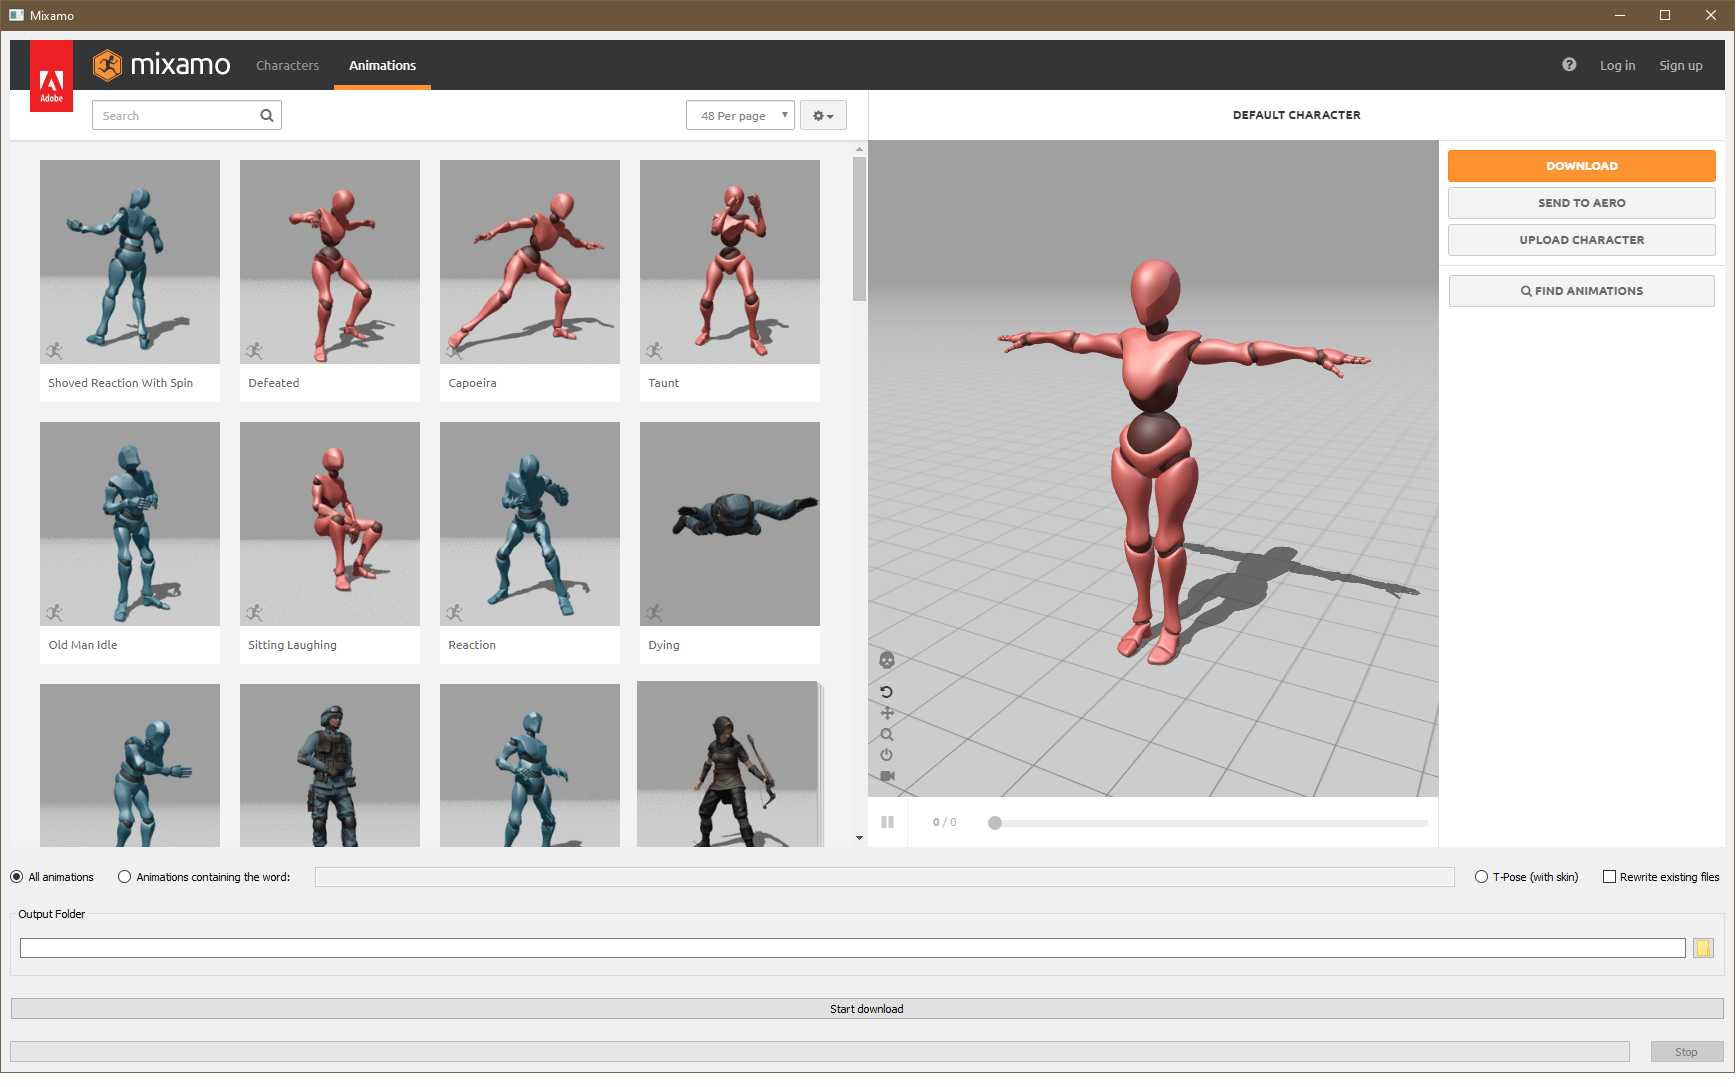
\includegraphics[width=0.7\textwidth]{Imagenes/Bitmap/caputra-mixamo-downloader.png}
    \caption{Herramienta Mixamo Downloader Arreglada}
    \label{fig:mixamo-downloader}
\end{figure}

Una vez realizados los cambios, se descargaron las animaciones disponibles en Mixamo para los gestos que se querían usar. El resultado de estas descargas se puede ver en el dataset \cite{raw-mixamo-animations}.

Las animaciones descargadas tienen un formato \gls{FBX}, por lo que era necesario pasarlas a un formato que puedan usar los modelos de \gls{ia}.
Para ello se decidió pasar la información relevante de los huesos en la toda la animación (su posición y rotación en cada frame) a un archivo CSV, donde cada columna iba a ser esta información y cada fila un frame de la animación. En la tabla \ref{tab:cabecera-csv-completa} se puede ver la cabecera para los CSV. En la siguiente tabla (\ref{tab:cabecera-csv-incompleta}) se puede ver un ejemplo de los valores que se guardan de un punto concreto del traje.

\begin{longtblr}[
        caption={Cabecera del \gls{csv} de cada animación, en órden descendente y de izquierda a derecha (incompleta).},
        label={tab:cabecera-csv-incompleta}
    ]{
        colspec={|l|l|l|},
        rowhead=1,
        hlines,
        row{even}={gray9},
        cells   = {font=\footnotesize\linespread{0.84}\selectfont},
    }
    Robot\_Hips\_posx &
    Robot\_Hips\_posy &
    Robot\_Hips\_posz   \\
    Robot\_Hips\_rotx &
    Robot\_Hips\_roty &
    Robot\_Hips\_rotz   \\
    ...               &
    ...               &
    ...                 \\
\end{longtblr}

Como no es viable ni escalable meter todas las animaciones a un proyecto de Unity ni crear un \gls{Animator} con todas estas se ideó una herramienta en Unity que se metiese todas las animaciones y construía el Animator en tiempo de ejecución.

\subsection{Carga mediante asset bundles}
En un principio se pensó en usar los assets bundles para cargar las animaciones.
Los assets bundles son archivos de Unity que contienen archivos serializados (cualquier asset para un videojuego menos código) y pueden cargarse en tiempo de ejecución.
Finalmente se descartó la idea de usar este tipo de archivos, ya que necesitan construirse en un proyecto de Unity, por lo que no solucionaba el problema de meter las animaciones a mano a un proyecto de Unity

\subsection{Carga mediante Asset Database}
Finalmente se decidió usar Asset Database para la carga automática de las animaciones.
Asset Database es una API de Unity que permiten trabajar con assets, siempre y cuando estén incluidos en el proyecto aunque no necesariamente cargados.
Para suplir la condición de que estuviesen incluidos en el proyecto se hizo un script que descargaba las animaciones, separadas por carpetas cuyo nombre era el tipo de gesto, desde la base de datos de Kaggle hacia la carpeta ``Resources'' del proyecto y ejecutaba desde línea de comandos el editor del proyecto.

Una vez las animaciones estuviesen descargadas en la carpeta de ``Resources'' del proyecto se busca iterativamente por la carpeta para cargar las animaciones y guardarse la relación entre el tipo de gesto y la animación.
Una vez completado empieza la ejecución de las animaciones.

Esta ejecución consiste en cargar la animación en la máquina de estados del \gls{Animator} gracias a un componente llamado ``Animator Override Controller'', que permite cambiar el clip de animación de una instancia del \gls{Animator} sin cambiar la lógica de su máquina de estados.
Cuando empieza la animación se crea un \gls{csv} con el formato ``Animación\_Número de animación.csv'' y empieza su ejecución.
Una vez finalizada la ejecución de una animación se cierra el \gls{csv} y se busca la siguiente animación. Se puede ver un ejemplo de todo este proceso en un timelapse de la ejecución de la herramienta\footnote{Enlace al timelapse completo a x4 de tiempo \url{https://youtu.be/NOawMoaG98M}}, también se deja una captura del mismo para ver el funcionamiento de la herramienta en el editor de Unity en la figura \ref{fig:frame-timelapse}, donde se puede ver al avatar ``Remy'' en mitad de una animación de baile. Este avatar lleva a cabo las animaciones del dataset para, en cada frame de ejecución, convertir sus coordenadas al \gls{csv} correspondiente.

\begin{figure}[H]
    \centering
    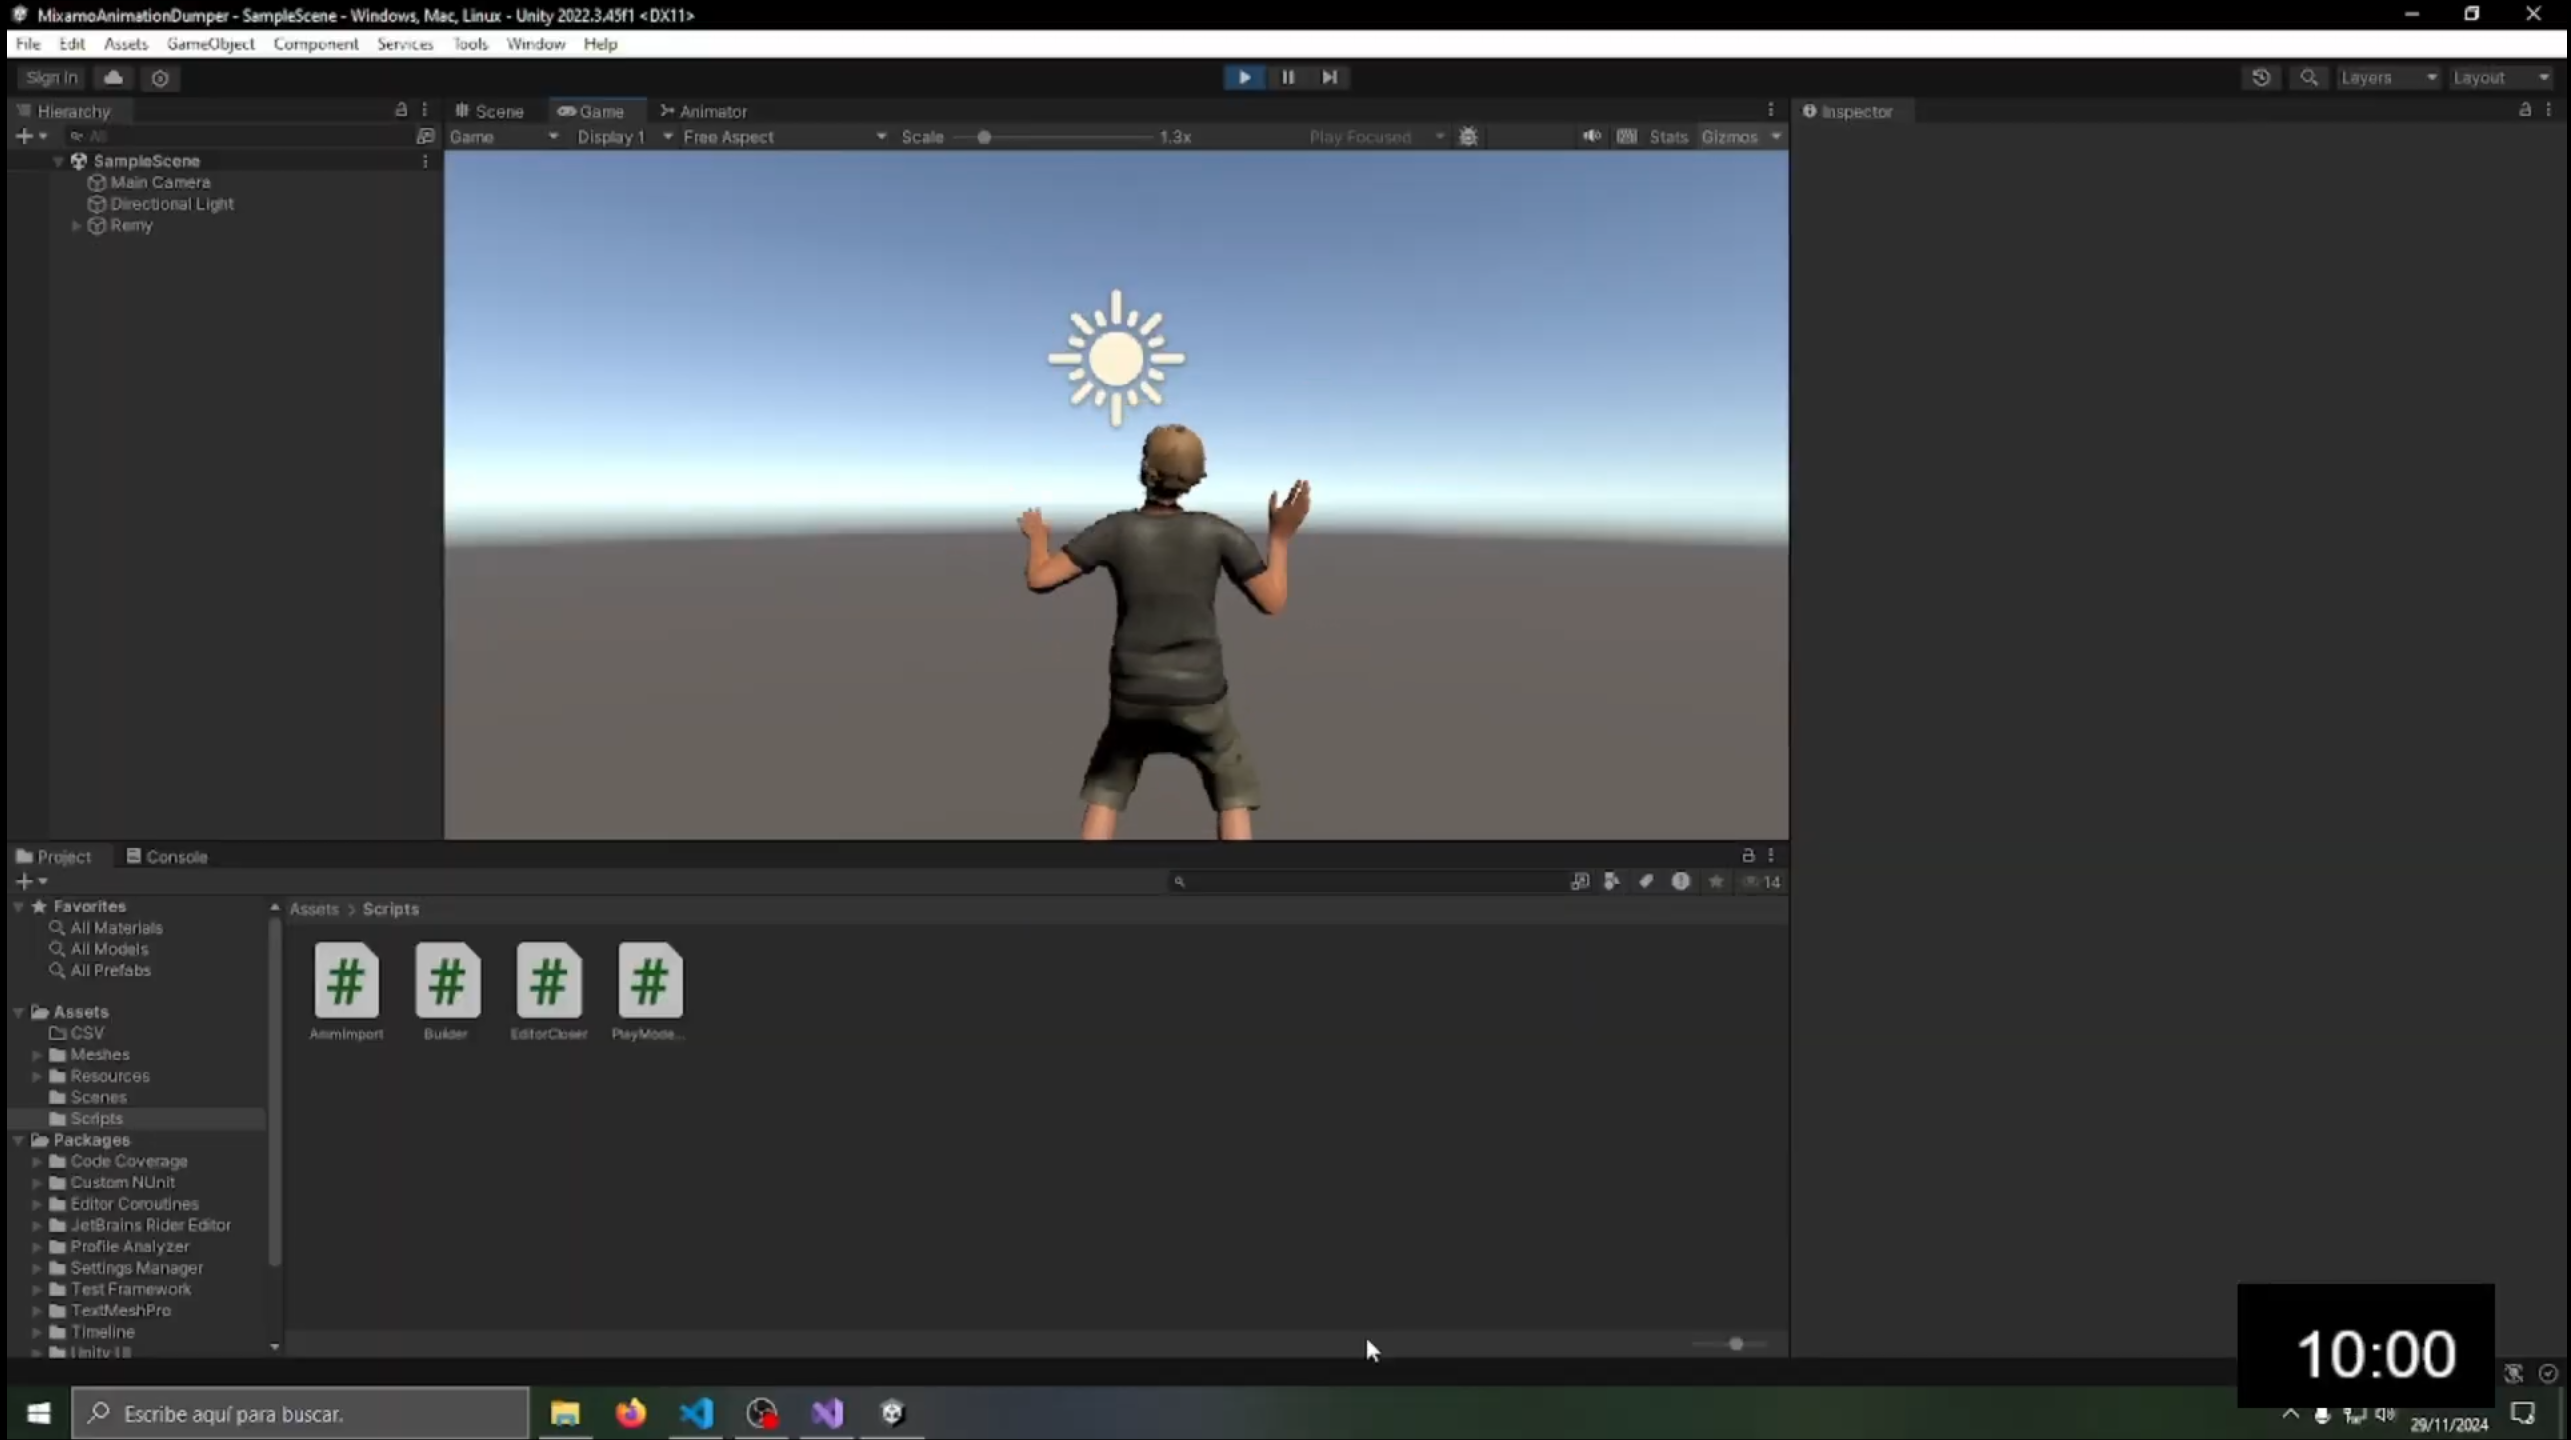
\includegraphics[width=0.7\textwidth]{Imagenes/Bitmap/remy_bailon.png}
    \caption{Frame de un \textit{timelapse} de la ejecución de la herramienta}
    \label{fig:frame-timelapse}
\end{figure}

En la figura \ref{fig:MixamoDumper} se puede ver un diagrama de flujo del funcionamiento de esta herramienta, mientras que el código de la misma es público\footnote{Enlace al repositorio de la herramienta: \url{https://github.com/FratosVR/Mixamo-Animation-Dumper}} y se puede ver en el apéndice \ref{appendix:MixamoDumperCode}.

El número de animaciones que se consiguieron grabar se puede ver en la figura \ref{fig:AnimacionesBruto}, donde se puede observar un desbalanceo de algunas animaciones (bailar o pelear) frente a otras (saludar o señalar).

Al finalizar todas las animaciones se cierra el editor de Unity y se procesan los CSV resultantes.

La ventaja de hacer esta herramienta es que es independiente del número de gestos y de animaciones por cada gesto, lo que hace que esta herramienta haga escalable el caso de que se quieran introducir o quitar gestos.

\begin{figure}[H]
    \centering
    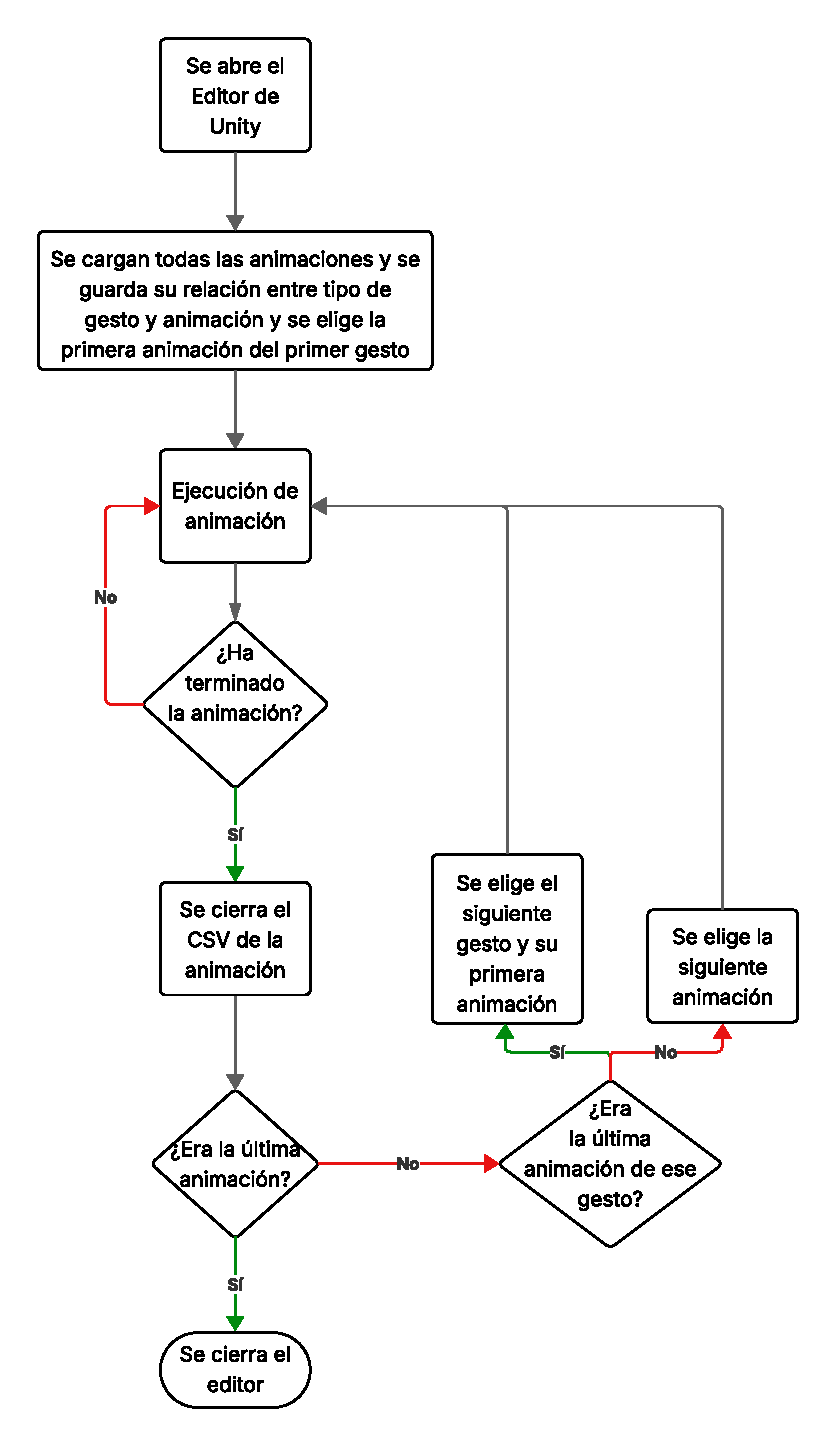
\includegraphics[width=0.7\textwidth]{Imagenes/Vectorial/FlujoMixamoDumper.pdf}
    \caption{Diagrama de flujo de la herramienta que carga y ejecuta las animaciones de Mixamo en tiempo de ejecución, llamada Mixamo Dumper}
    \label{fig:MixamoDumper}
\end{figure}


\begin{figure}[H]
    \centering
    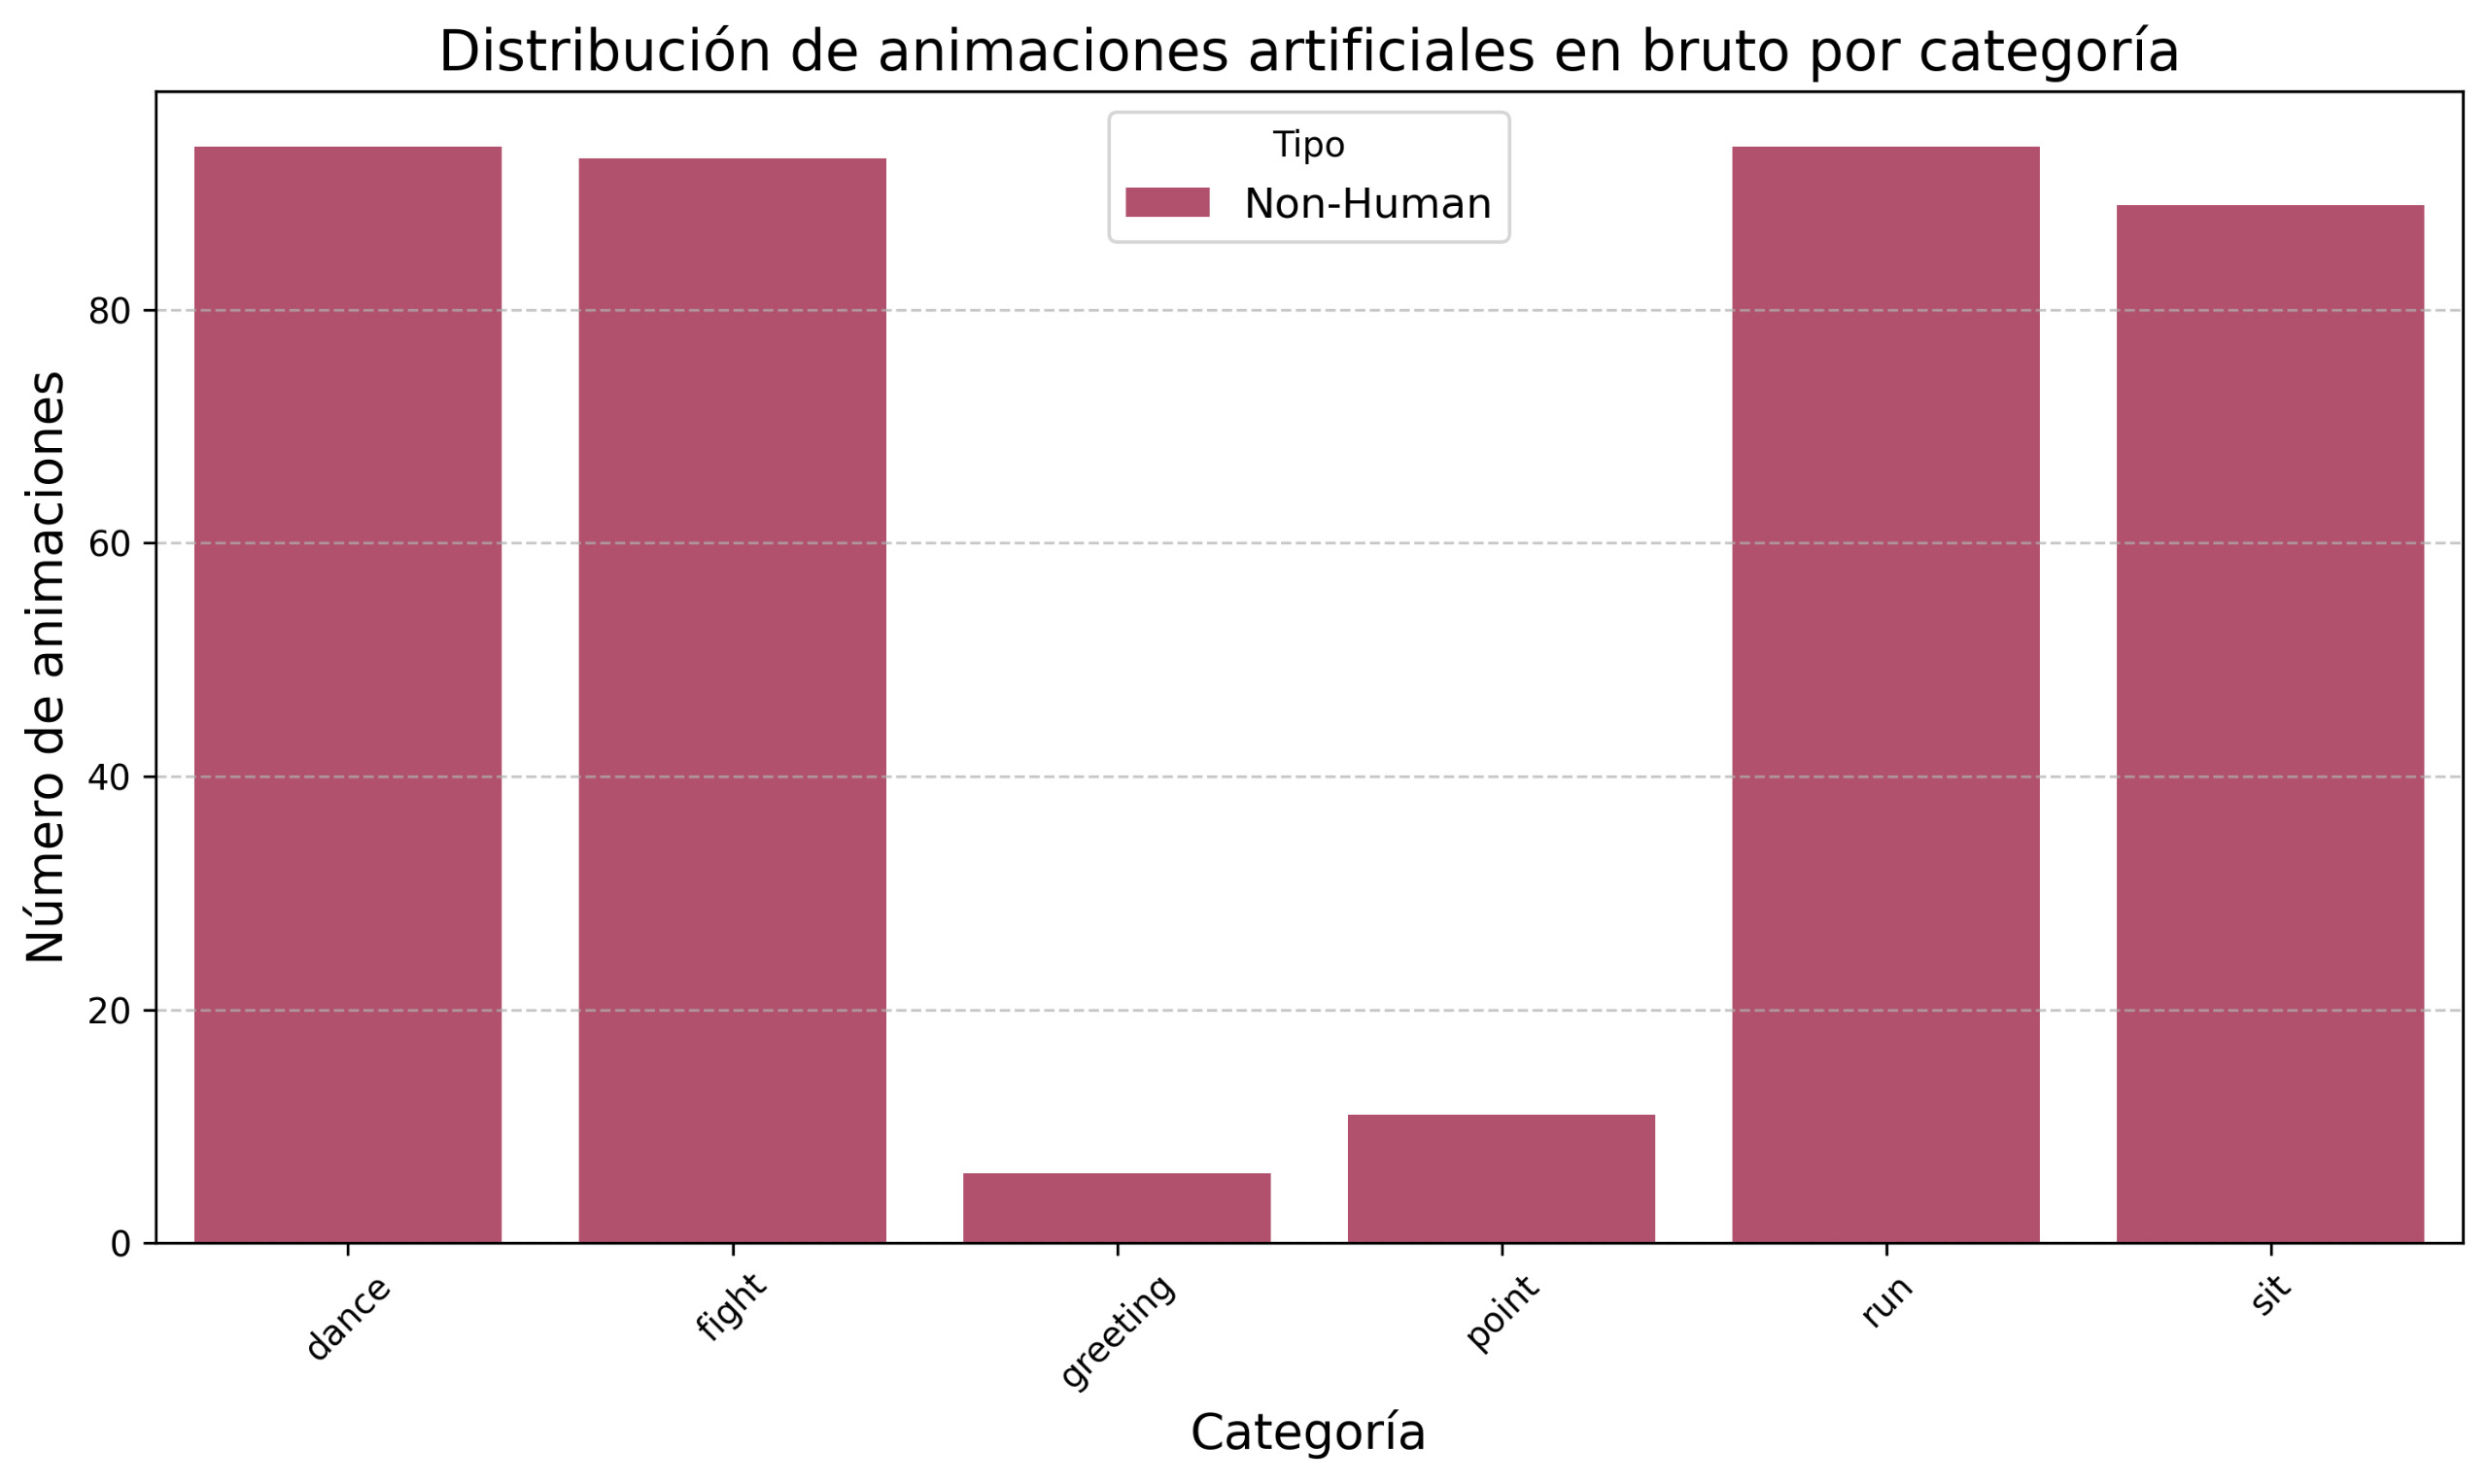
\includegraphics[width=0.8\textwidth]{Imagenes/Bitmap/AnimacionesBruto.jpeg}
    \caption{Número de animaciones conseguidas gracias a la herramienta divididas por tipo de gesto}
    \label{fig:AnimacionesBruto}
\end{figure}


\subsection{Tratamiento de CSV resultantes}

Los \glspl{csv} restantes se copiaron en un nuevo \textit{dataset} de Kaggle en una carpeta llamada ``full\_animations''. Una vez subidos estos datos, se creó una clase en Python para estandarizar estos \glspl{csv}. Los datos se estandarizaron con el siguiente criterio:
\begin{itemize}
    \item Todas las animaciones deben de tener el mismo número de frames. Para ello se estandarizará la duración a 90 frames que es el número de \gls{fps} que usan las gafas de \gls{vr} de Meta Quest 2 y la herramienta Mixamo Animation Dumper.
    \item Las animaciones que duraran más de 90 frames se dividen en varias animaciones de 90 frames o menos.
    \item Las animaciones que duraran menos de 90 frames se repiten desde el inicio hasta completar los 90 frames.
    \item Las animaciones que no lleguen a 10 frames se consideran inválidas y se eliminan.
\end{itemize}

Este proceso se puede ver de manera más visual en la figura \ref{fig:data_cleaner} y se puede ver el diagrama de la clase DataLoader \footnote{Enlace de la herramienta \url{https://github.com/FratosVR/Models/src/DataLoader.py}} en la figura \ref{fig:data_loader}, algunas de las funciones de esta clase se verán en los próximos apartados.

\begin{figure}[H]
    \centering
    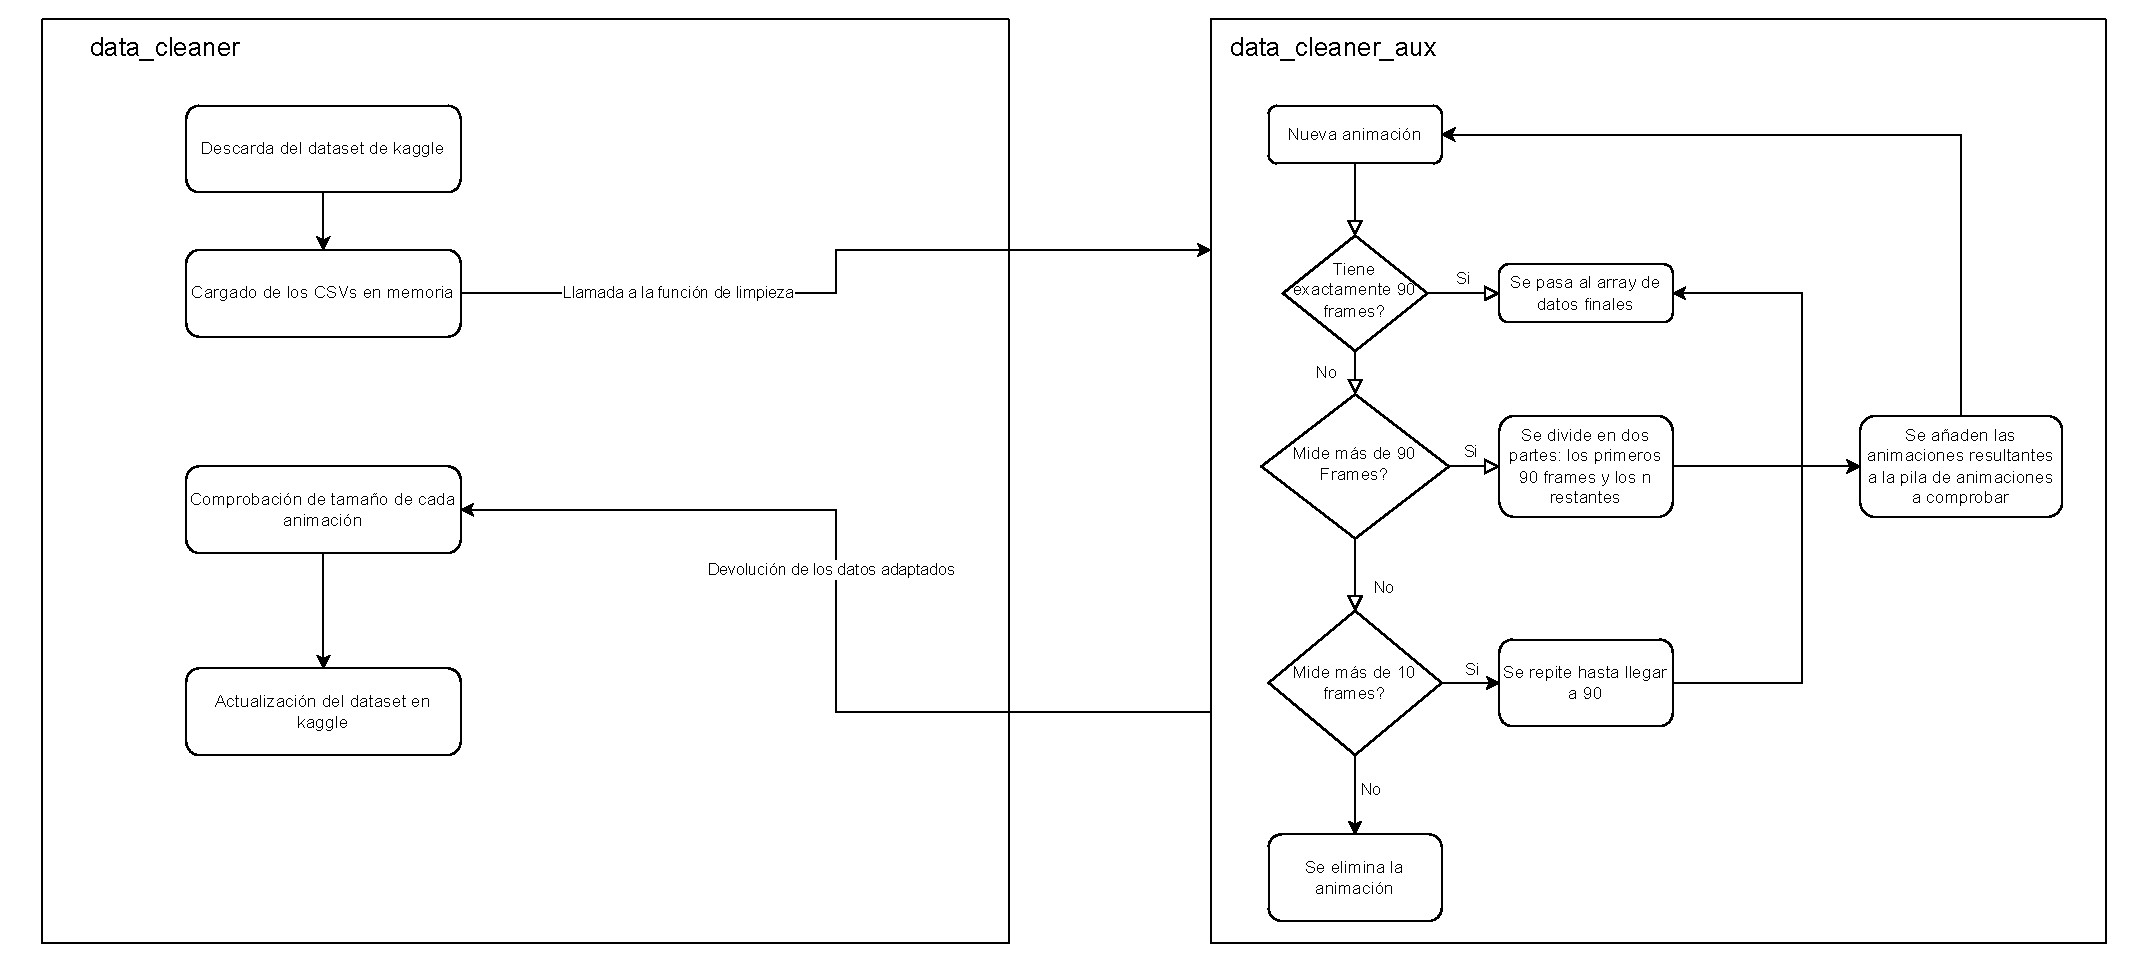
\includegraphics[width=0.8\textwidth]{Imagenes/Vectorial/data_cleaner.pdf}
    \caption{Diagrama de flujo del proceso de limpieza de datos (funciones data\_cleaner y data\_cleaner\_aux de la clase DataLoader)}
    \label{fig:data_cleaner}
\end{figure}

\begin{figure}[H]
    \centering
    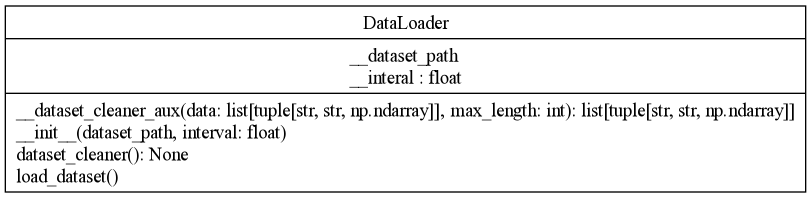
\includegraphics[width=0.9\textwidth]{Imagenes/Bitmap/DataLoader_UML.png}
    \caption{Diagrama de la clase DataLoader}
    \label{fig:data_loader}
\end{figure}

El resultado de la estandarización se puede ver en la figura \ref{fig:AnimacionesEstandar}, donde se puede ver una diferencia notable entre las animaciones de bailar frente al resto.

\begin{figure}[H]
    \centering
    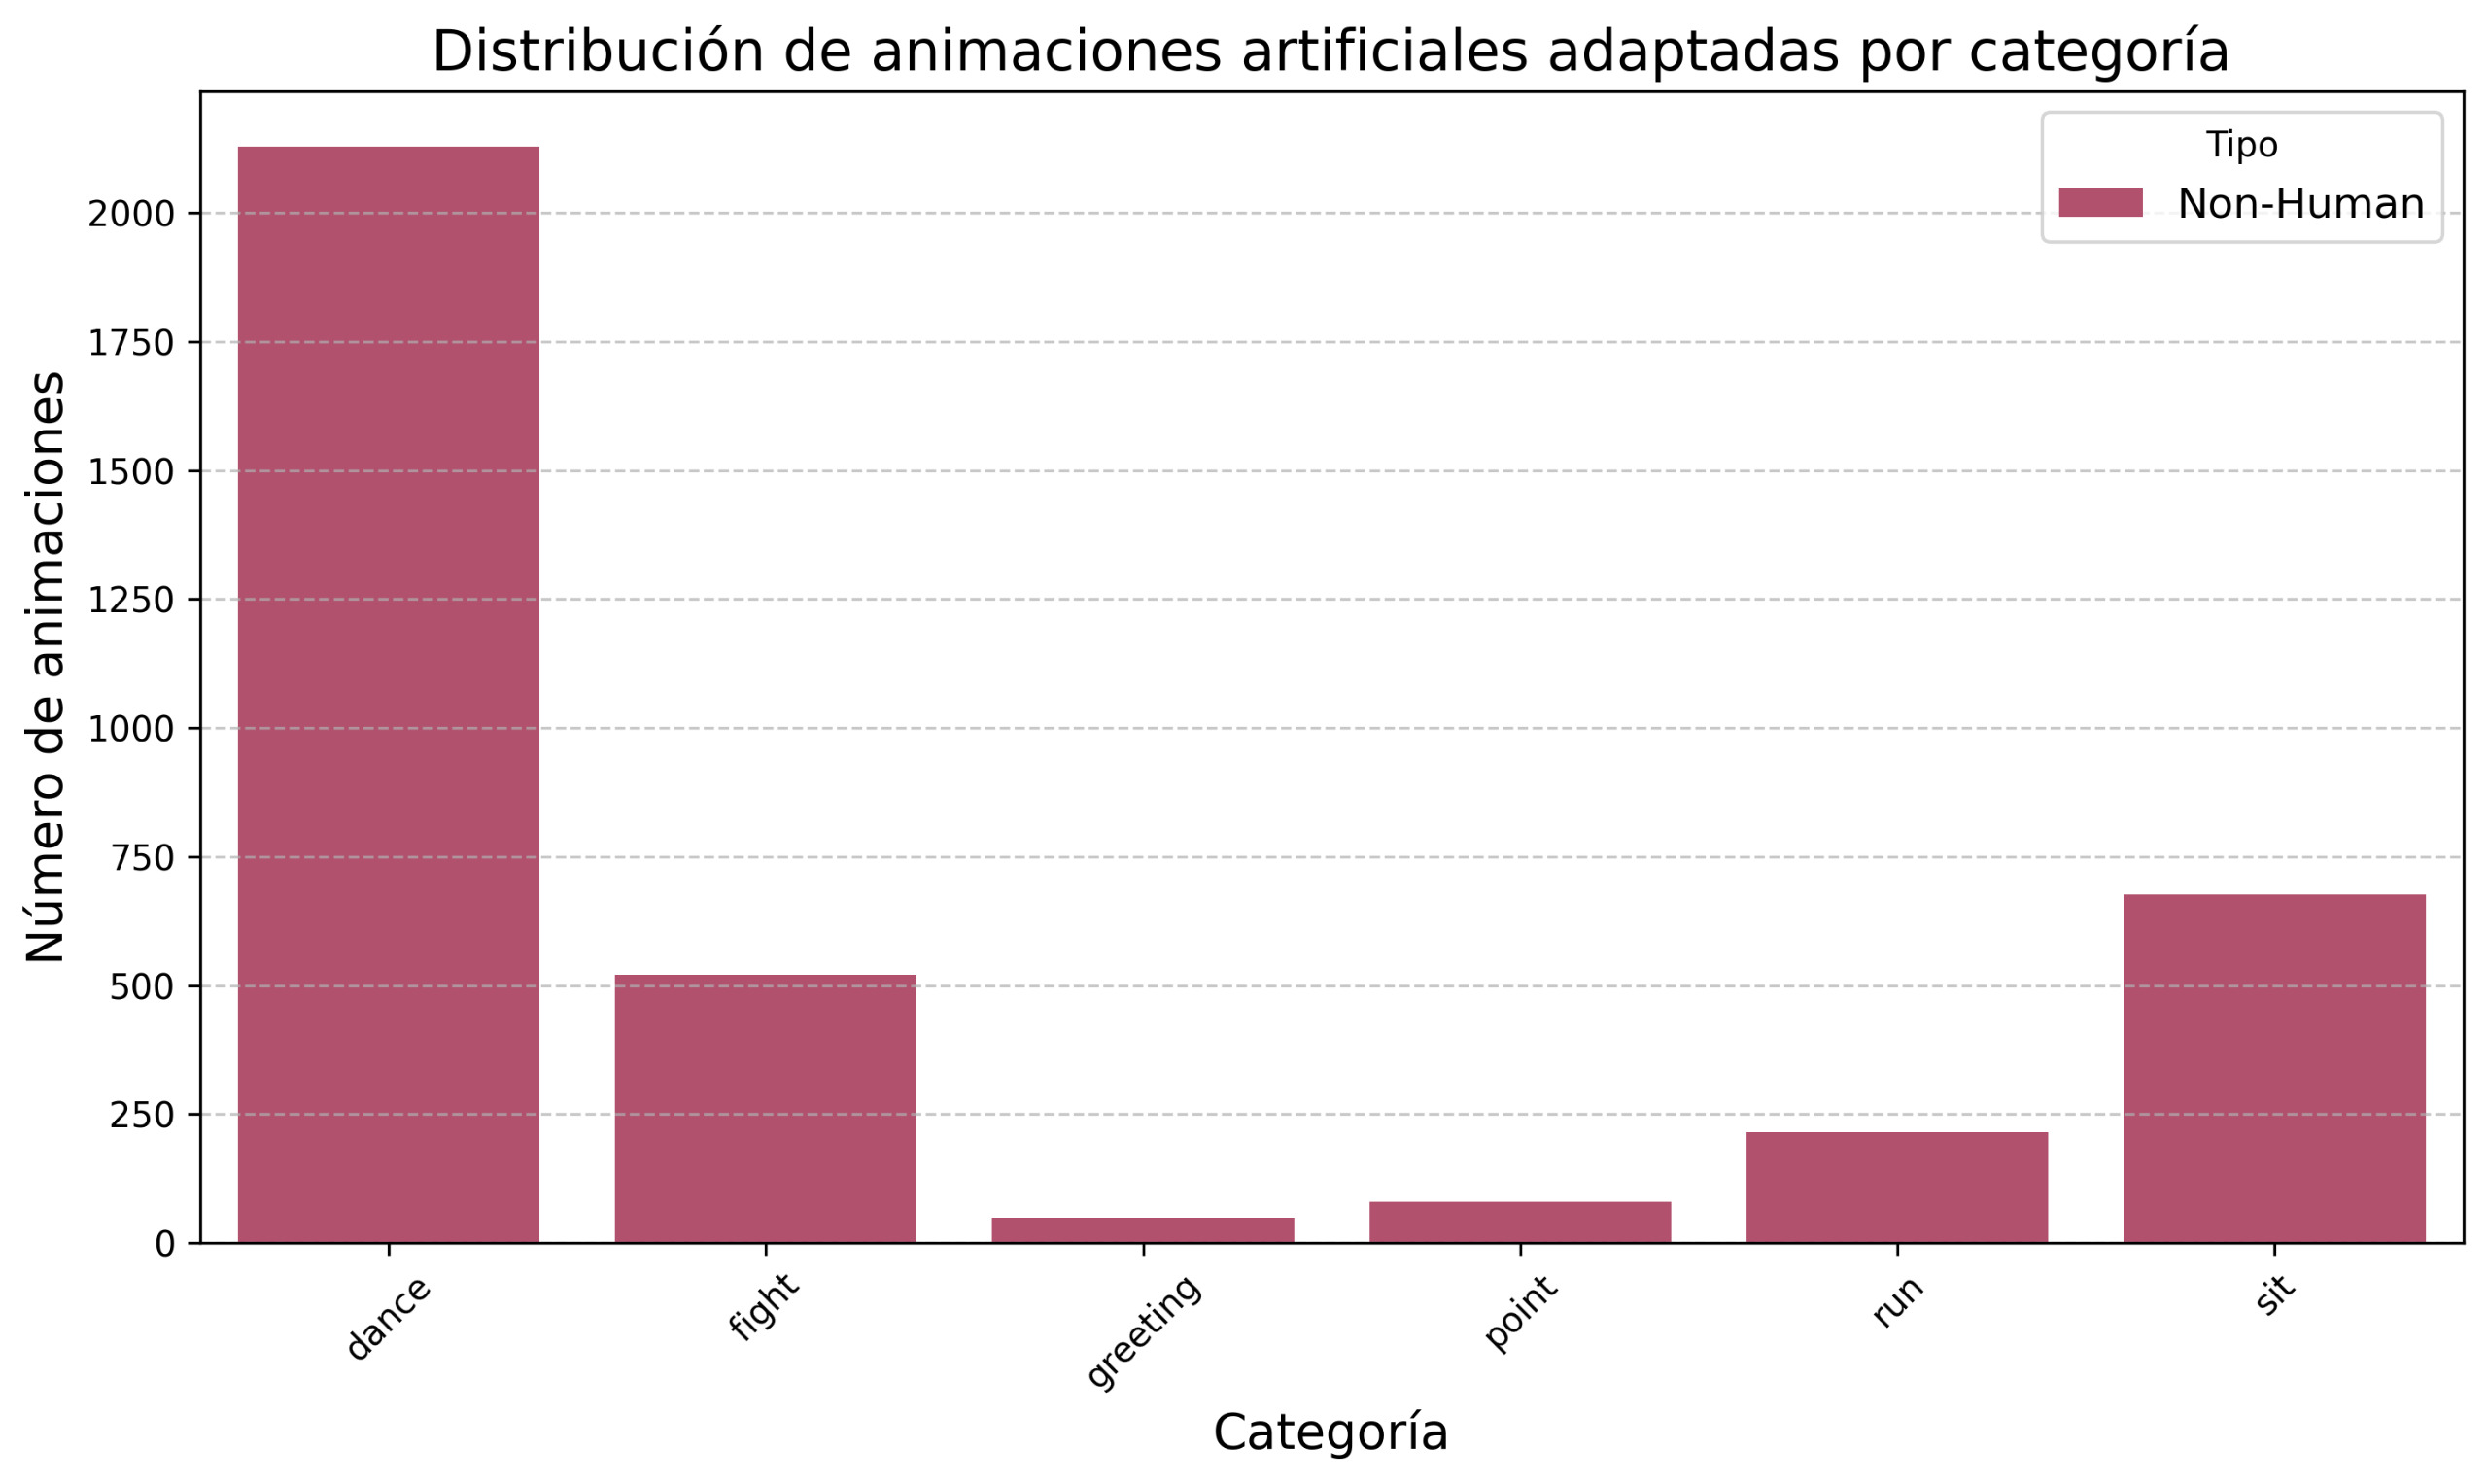
\includegraphics[width=0.8\textwidth]{Imagenes/Bitmap/AnimacionesEstandarizadas.jpeg}
    \caption{Número de animaciones estandarizadas divididas por tipo de gesto}
    \label{fig:AnimacionesEstandar}
\end{figure}
